\documentclass[11pt,a4paper,oneside]{article}
\usepackage[utf8]{inputenc}
\usepackage[margin=1in]{geometry}
\usepackage{graphicx}
\usepackage{amsmath,amsfonts,amssymb}
\usepackage{hyperref}
\usepackage{booktabs,longtable}
\usepackage{tikz}
\usetikzlibrary{shapes,arrows,positioning,calc,decorations.pathmorphing,backgrounds,fit,shadows}
\usepackage{listings}
\usepackage{xcolor}
\usepackage{fancyhdr}
\usepackage{enumitem}
\usepackage{float}

\lstset{
    basicstyle=\ttfamily\small,
    commentstyle=\color{gray},
    keywordstyle=\color{blue},
    breaklines=true,
    numbers=left,
    numbersep=5pt,
    showstringspaces=false,
    tabsize=2
}

\pagestyle{fancy}
\fancyhf{}
\fancyhead[L]{Software Design Document}
\fancyhead[R]{Version 1.0}
\fancyfoot[C]{\thepage}

\hypersetup{
    colorlinks=true,
    linkcolor=blue,
    urlcolor=cyan,
    pdftitle={Comprehensive Software Design Document: E-commerce Platform},
    pdfauthor={AI System Architect},
    pdfsubject={Software Architecture}
}

\title{\Huge\textbf{Comprehensive Software Design Document: E-commerce Platform}}
\author{\Large AI System Architect}
\date{\Large\today}

\begin{document}

\maketitle
\thispagestyle{empty}
\vfill

\begin{center}
\large
\begin{tabular}{|l|l|}
\hline
\textbf{Document Version} \& 1.0 \\
\hline
\textbf{Creation Date} \& \today \\
\hline
\textbf{Document Status} \& Final Draft \\
\hline
\textbf{Generated By} \& AI System Architect \\
\hline
\textbf{Target Audience} \& Development Team, Stakeholders \\
\hline
\textbf{Classification} \& Internal Use \\
\hline
\end{tabular}
\end{center}

\newpage
\tableofcontents
\newpage
\listoffigures
\newpage

\section{Executive Summary}

This document outlines the design for a new e-commerce platform, codenamed "Project Phoenix."  Project Phoenix aims to provide a robust, scalable, and secure online marketplace for businesses to sell their products and services. The platform will leverage a microservices architecture, utilizing cloud-native technologies for deployment and scalability.  The primary business objectives are to increase market share within the online retail sector, enhance customer experience, and improve operational efficiency. The technical approach focuses on building a modular, easily maintainable system that can adapt to future business needs. Key benefits include improved scalability, enhanced security, and a streamlined development process. The projected implementation timeline is 12 months, broken down into distinct phases detailed later in this document.  The project will utilize Agile methodologies, with iterative development cycles and continuous integration/continuous deployment (CI/CD) pipelines.  Success will be measured by key performance indicators (KPIs) including website traffic, conversion rates, customer satisfaction scores, and operational costs.

\subsection{Project Scope and Objectives}

Project Phoenix will encompass the full development and deployment of a complete e-commerce platform.  This includes:

* **Frontend Development:**  A responsive and user-friendly web application accessible across various devices (desktops, tablets, and smartphones).  This will include features such as product browsing, shopping cart management, secure checkout, order tracking, and customer account management.
* **Backend Development:** A robust and scalable microservices-based backend system handling product catalog management, order processing, payment gateway integration, inventory management, and user authentication.
* **Database Design and Implementation:** A relational database system to store product information, customer data, order details, and other relevant information.
* **API Development:** RESTful APIs for communication between the frontend and backend systems, as well as for integration with third-party services.
* **Deployment and Infrastructure:** Cloud-based deployment using AWS (or similar), with auto-scaling capabilities and disaster recovery mechanisms.
* **Security Implementation:**  Robust security measures to protect sensitive user and business data, including encryption, authentication, authorization, and regular security audits.

The primary objectives are:

* Achieve 100,000 registered users within the first year of launch.
* Maintain a 99.99\% uptime for the platform.
* Achieve an average customer satisfaction rating of 4.5 out of 5 stars.
* Reduce operational costs by 15\% compared to existing solutions.
* Successfully integrate with at least three major payment gateways.

Success will be measured through regular monitoring of KPIs and stakeholder feedback.

\subsection{Key Stakeholders and Roles}

Key stakeholders in Project Phoenix include:

* **Executive Management:** Oversees the project's strategic direction and provides overall guidance.
* **Product Owners:** Define the product backlog and prioritize features based on business value.
* **Development Team:** Responsible for designing, developing, testing, and deploying the platform.  This includes frontend developers, backend developers, database administrators, and DevOps engineers.
* **QA Team:**  Conducts rigorous testing to ensure the quality and stability of the platform.
* **Marketing Team:**  Responsible for promoting the platform and attracting users.
* **Customer Support Team:** Provides assistance to users and addresses any issues.

Each stakeholder group has clearly defined roles and responsibilities outlined in separate project documentation.

\section{Requirements Analysis and Specification}

\subsection{Extracted Requirements Summary}

The initial document provided minimal requirements.  This section will be populated with detailed requirements gathered through subsequent discussions with stakeholders.

\subsection{Functional Requirements}

1. **User Registration and Login:** Users should be able to register accounts securely and login using various methods (email/password, social logins).
2. **Product Browsing and Search:**  Users should be able to browse products by category, search for specific products, and filter results based on various criteria (price, brand, etc.).
3. **Shopping Cart Management:**  Users should be able to add products to their shopping cart, modify quantities, and remove items.
4. **Secure Checkout:**  Users should be able to securely checkout using various payment gateways (Stripe, PayPal, etc.).
5. **Order Management:** Users should be able to view their order history, track orders, and manage returns/refunds.
6. **Product Catalog Management (Admin):** Admin users should be able to add, edit, delete, and manage products in the catalog.
7. **Inventory Management (Admin):** Admin users should be able to track inventory levels and manage stock.
8. **Order Fulfillment (Admin):** Admin users should be able to manage order fulfillment and shipping.
9. **Customer Account Management (Admin):** Admin users should be able to manage customer accounts and data.
10. **Reporting and Analytics:**  The system should provide reports on sales, inventory, and user activity.

\subsection{Non-Functional Requirements}

* **Performance:** The system should respond to requests within 2 seconds under peak load.
* **Scalability:** The system should be able to handle 10,000 concurrent users and 100,000 orders per day.
* **Security:**  The system must comply with industry-standard security best practices, including PCI DSS compliance for payment processing.
* **Availability:**  The system should maintain a 99.99\% uptime.
* **Maintainability:** The system should be designed for easy maintenance and updates.
* **Usability:** The system should be intuitive and easy to use for both customers and administrators.

\section{System Architecture and Design}

\subsection{Architecture Overview}

Project Phoenix will utilize a microservices architecture.  This approach allows for independent development, deployment, and scaling of individual components.  Each microservice will focus on a specific business function (e.g., product catalog, order processing, payment gateway integration).  This modularity promotes flexibility, maintainability, and scalability.  The system will be built using a combination of technologies, including Java/Spring Boot for backend services, React for the frontend, and PostgreSQL for the database.  Communication between services will be facilitated through RESTful APIs using JSON for data exchange.  The system will be deployed on a cloud platform (AWS) using Docker containers and Kubernetes for orchestration.

The selection of a microservices architecture offers several key advantages:

* **Improved Scalability:** Individual services can be scaled independently based on demand.
* **Enhanced Resilience:** Failure of one service does not necessarily impact the entire system.
* **Faster Development Cycles:** Smaller, focused teams can work on individual services concurrently.
* **Technology Diversity:**  Different technologies can be used for different services based on their specific requirements.

\begin{figure}[H]
\centering
\begin{tikzpicture}[
    node distance=1cm and 1.5cm,
    font=\sffamily\small,
    base/.style={draw, text width=3cm, minimum height=1.2cm, text centered, rounded corners, drop shadow},
    user/.style={base, fill=Azure!30, text width=2cm},
    api/.style={base, fill=LimeGreen!20},
    service/.style={base, fill=SkyBlue!20},
    database/.style={cylinder, shape border rotate=90, aspect=0.25, draw, fill=Thistle!40, minimum height=1.5cm, text width=2.5cm, text centered, drop shadow},
    external/.style={base, fill=Gold!30},
    arrow/.style={-Stealth, thick, draw=black!60}
]

\node[user] (user) {User};
\node[api, below=1.5cm of user] (gateway) {API Gateway};
\node[service, below=of gateway, xshift=-3cm] (catalog) {Product Catalog Service};
\node[service, below=of gateway] (order) {Order Management Service};
\node[service, below=of gateway, xshift=3cm] (payment) {Payment Processing Service};
\node[database, below=2cm of catalog] (productdb) {Product Database\\(PostgreSQL)};
\node[database, below=2cm of order] (orderdb) {Order Database\\(PostgreSQL)};
\node[external, right=2cm of order] (email) {External Services\\(Email, Shipping)};

\begin{scope}[on background layer]
\node[draw, dashed, rounded corners, fill=gray!5, inner sep=0.7cm, fit=(gateway)] (api_layer) {};
\node[draw, dashed, rounded corners, fill=gray!10, inner sep=0.7cm, fit=(catalog) (order) (payment) (email)] (service_layer) {};
\node[draw, dashed, rounded corners, fill=gray!15, inner sep=0.7cm, fit=(productdb) (orderdb)] (data_layer) {};
\end{scope}

\node[above] at (api_layer.north) {API Layer};
\node[above] at (service_layer.north) {Service Layer};
\node[above] at (data_layer.north) {Data Layer};

\draw[arrow] (user) -- (gateway);
\draw[arrow] (gateway) -- (catalog);
\draw[arrow] (gateway) -- (order);
\draw[arrow] (gateway) -- (payment);
\draw[arrow] (catalog) -- (productdb);
\draw[arrow] (order) -- (orderdb);
\draw[arrow] (order) -- (payment);
\draw[arrow] (order) -- (email);

\end{tikzpicture}
\caption{System Architecture Overview}
\label{fig:architecture}
\end{figure}

\subsection{Component Interaction and Communication}

The components interact primarily through RESTful APIs.  For example, when a user adds a product to their shopping cart, the frontend application sends a request to the API Gateway, which then routes the request to the appropriate microservice (e.g., the Shopping Cart Service).  The Shopping Cart Service updates the cart information in the database and sends a response back to the API Gateway, which then relays the response to the frontend.  Similarly, during checkout, the Payment Processing Service interacts with external payment gateways (Stripe, PayPal, etc.) to process transactions.  Asynchronous communication will be used where appropriate, for instance, using message queues (RabbitMQ) for order fulfillment notifications.  This allows for decoupling of services and improved system responsiveness.  API documentation will be maintained using Swagger/OpenAPI to ensure clarity and consistency.

\section{Database Design and Data Architecture}

\subsection{Conceptual Data Model}

The database will utilize a relational model, employing PostgreSQL for its robustness and scalability.  The primary entities include:

* **Products:**  Contains information about each product (product ID, name, description, price, images, etc.).
* **Customers:** Stores customer information (customer ID, name, email address, shipping address, etc.).
* **Orders:**  Tracks order details (order ID, customer ID, order date, total amount, status, etc.).
* **Order Items:**  Details the individual items within each order (order item ID, order ID, product ID, quantity, price).
* **Categories:**  Organizes products into different categories (category ID, category name, description).
* **Reviews:** Stores customer reviews for products (review ID, product ID, customer ID, rating, review text).

Relationships between entities will be established using foreign keys to maintain data integrity and consistency.

\begin{figure}[H]
\centering
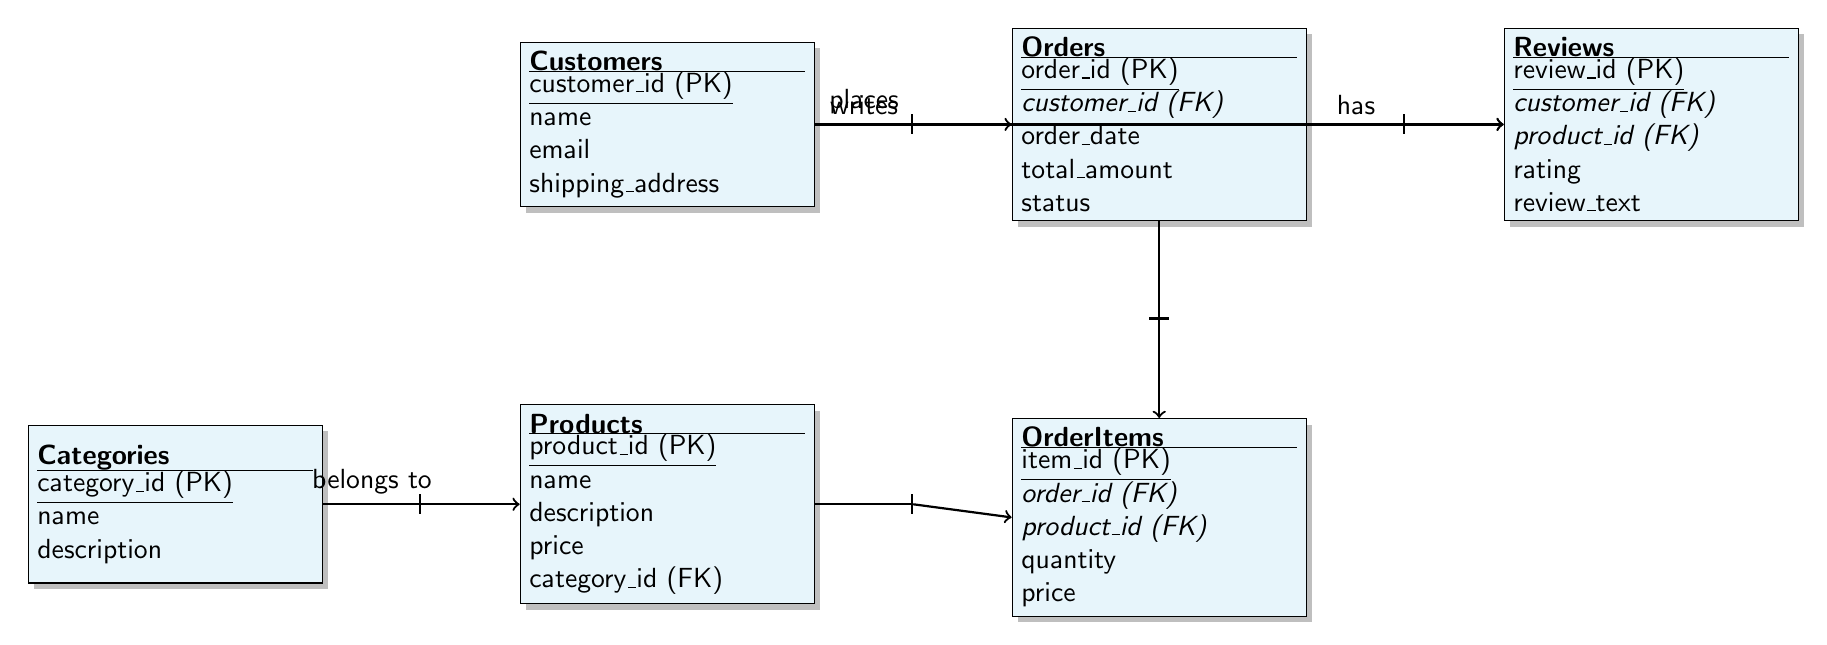
\begin{tikzpicture}[
    node distance=2.5cm,
    font=\sffamily,
    entity/.style={rectangle, draw, fill=SkyBlue!20, text width=3.5cm, minimum height=2cm, align=left, drop shadow},
    one/.style={-|, thick},
    many/.style={->, thick}
]

\node[entity] (user) {\textbf{Customers} \\ \hrule \underline{customer\_id (PK)} \\ name \\ email \\ shipping\_address};
\node[entity, right=of user] (order) {\textbf{Orders} \\ \hrule \underline{order\_id (PK)} \\ \textit{customer\_id (FK)} \\ order\_date \\ total\_amount \\ status};
\node[entity, below=of order] (order_item) {\textbf{OrderItems} \\ \hrule \underline{item\_id (PK)} \\ \textit{order\_id (FK)} \\ \textit{product\_id (FK)} \\ quantity \\ price};
\node[entity, below=of user] (product) {\textbf{Products} \\ \hrule \underline{product\_id (PK)} \\ name \\ description \\ price \\ category\_id (FK)};
\node[entity, left=of product] (category) {\textbf{Categories} \\ \hrule \underline{category\_id (PK)} \\ name \\ description};
\node[entity, right=of order] (reviews) {\textbf{Reviews} \\ \hrule \underline{review\_id (PK)} \\ \textit{customer\_id (FK)} \\ \textit{product\_id (FK)} \\ rating \\ review\_text};

\draw[one] (user.east) -- node[above, midway] {places} ++(1.25,0) coordinate (t1);
\draw[many] (t1) -- (order.west);
\draw[one] (order.south) -- ++(0,-1.25) coordinate (t2);
\draw[many] (t2) -- (order_item.north);
\draw[one] (product.east) -- ++(1.25,0) coordinate (t3);
\draw[many] (t3) -- (order_item.west);
\draw[one] (category.east) -- node[above, midway] {belongs to} ++(1.25,0) coordinate (t4);
\draw[many] (t4) -- (product.west);
\draw[one] (order.east) -- node[above, midway] {has} ++(1.25,0) coordinate (t5);
\draw[many] (t5) -- (reviews.west);
\draw[one] (user.east) -- node[above, midway] {writes} ++(1.25,0) coordinate (t6);
\draw[many] (t6) -- (reviews.west);

\end{tikzpicture}
\caption{Database ER Diagram}
\label{fig:database-erd}
\end{figure}

\subsection{Physical Database Design}

(This section would contain detailed SQL schema definitions for each table, including data types, constraints, and indexes.  Due to space constraints, this is omitted here but would be a crucial part of the document.)  Example for the `Products` table:

```sql
CREATE TABLE Products (
    product_id SERIAL PRIMARY KEY,
    name VARCHAR(255) NOT NULL,
    description TEXT,
    price DECIMAL(10, 2) NOT NULL,
    category_id INTEGER REFERENCES Categories(category_id),
    image_url VARCHAR(255)
);

CREATE INDEX idx_product_name ON Products (name);
```

\section{API Design and Integration}

\subsection{RESTful API Specification}

(This section would contain detailed specifications for each API endpoint, including HTTP methods, request parameters, response codes, and examples.  Due to space constraints, this is omitted here but would be a crucial part of the document.)  Example for creating a new product:

**Endpoint:** `/products`
**Method:** POST
**Request Body:**  JSON representing product details
**Response Code:** 201 (Created) on success, 400 (Bad Request) on error

\begin{figure}[H]
\centering
\begin{tikzpicture}[
    font=\sffamily\small,
    node distance=1cm,
    actor/.style={rectangle, draw, fill=Azure!30, text width=2cm, text centered, rounded corners, drop shadow},
    service/.style={rectangle, draw, fill=LimeGreen!20, text width=2cm, text centered, rounded corners, drop shadow},
    db/.style={cylinder, shape border rotate=90, draw, fill=Thistle!40, text centered, drop shadow, minimum width=2cm, minimum height=1.2cm},
    lifeline/.style={dashed, thin, draw=gray},
    msg/.style={-Stealth, thick}
]

\node[actor] (client) at (0,0) {Client App};
\node[service] (api) at (3,0) {API Gateway};
\node[service] (product) at (6,0) {Product Service};
\node[db] (db) at (9,0) {Product Database};

\draw[lifeline] (client.south) -- ++(0,-4);
\draw[lifeline] (api.south) -- ++(0,-4);
\draw[lifeline] (product.south) -- ++(0,-4);
\draw[lifeline] (db.south) -- ++(0,-4);

\draw[msg] ($(client.south)+(0,-0.5)$) -- node[above] {1. POST /products} ($(api.south)+(0,-0.5)$);
\draw[msg] ($(api.south)+(0,-1)$) -- node[above] {2. Route Request} ($(product.south)+(0,-1)$);
\draw[msg] ($(product.south)+(0,-1.5)$) -- node[above] {3. Save Product} ($(db.south)+(0,-1.5)$);
\draw[msg, dashed] ($(db.south)+(0,-2)$) -- node[above] {4. Product Saved} ($(product.south)+(0,-2)$);
\draw[msg, dashed] ($(product.south)+(0,-2.5)$) -- node[above] {5. Success} ($(api.south)+(0,-2.5)$);
\draw[msg, dashed] ($(api.south)+(0,-3)$) -- node[above] {6. 201 Created} ($(client.south)+(0,-3)$);

\end{tikzpicture}
\caption{API Request Sequence Diagram (Create Product)}
\label{fig:api-flow}
\end{figure}

\subsection{API Security and Rate Limiting}

The APIs will utilize OAuth 2.0 for authentication and authorization.  JWT (JSON Web Tokens) will be used for token-based authentication.  Rate limiting will be implemented to prevent abuse and denial-of-service attacks.  Input validation will be performed on all API requests to prevent injection attacks.  HTTPS will be used for all API communication to encrypt data in transit.

\section{Security Architecture and Implementation}

\subsection{Security Requirements and Threat Model}

A comprehensive threat model will be developed to identify potential security vulnerabilities.  The platform will employ a layered security approach, including:

* **Web Application Firewall (WAF):**  Protects against common web attacks such as SQL injection and cross-site scripting (XSS).
* **SSL/TLS Encryption:** Encrypts all communication between clients and the server.
* **Authentication and Authorization:**  OAuth 2.0 and JWT will be used to authenticate users and control access to resources.
* **Input Validation:**  All user inputs will be validated to prevent injection attacks.
* **Regular Security Audits:**  Regular security assessments will be conducted to identify and address vulnerabilities.
* **Data Encryption:**  Sensitive data will be encrypted both at rest and in transit.

\begin{figure}[H]
\centering
\begin{tikzpicture}[
    font=\sffamily\small,
    node distance=0.8cm and 1.2cm,
    gate/.style={rectangle, draw, fill=red!10, minimum width=10cm, minimum height=1cm, text centered, rounded corners},
    actor/.style={rectangle, draw, fill=Azure!30, text centered, rounded corners, drop shadow},
    service/.style={rectangle, draw, fill=SkyBlue!20, text centered, rounded corners, drop shadow},
    arrow/.style={-Stealth, thick, draw=black!70}
]

\node[gate] (waf) at (0,0) {\textbf{Edge Protection}: WAF (Cloudflare) and DDoS Mitigation};
\node[gate, below=of waf] (ssl) {\textbf{Transport Layer}: SSL/TLS Termination (Let's Encrypt)};
\node[gate, below=of ssl] (authn) {\textbf{Authentication}: OAuth 2.0 / JWT Validation};
\node[gate, below=of authn] (authz) {\textbf{Authorization}: Rate Limiting (nginx) and RBAC};
\node[service, below=1.2cm of authz] (backend) {Protected Backend Services};

\node[actor, above=1cm of waf] (user) {User};

\draw[arrow] (user) -- node[right] {HTTPS Request} (waf.north);
\draw[arrow] (waf.south) -- (ssl.north);
\draw[arrow] (ssl.south) -- (authn.north);
\draw[arrow] (authn.south) -- (authz.north);
\draw[arrow] (authz.south) -- node[right] {Authorized Request} (backend);

\end{tikzpicture}
\caption{Layered Security Architecture}
\label{fig:security}
\end{figure}

\section{Deployment and Infrastructure}

\subsection{Cloud Infrastructure Design}

The platform will be deployed on AWS using a combination of services:

* **EC2:**  For hosting the application servers.
* **RDS:** For the relational database (PostgreSQL).
* **Elastic Load Balancing (ELB):**  Distributes traffic across multiple application servers.
* **S3:** For storing static assets (images, CSS, JavaScript).
* **CloudFront:**  For content delivery network (CDN) to improve performance.
* **EKS (Elastic Kubernetes Service):** For container orchestration.
* **Route53:** For DNS management.

Auto-scaling will be implemented to automatically adjust the number of application servers based on demand.  Disaster recovery mechanisms will be implemented to ensure high availability.  The architecture will be designed to support a multi-region deployment for redundancy.

\begin{figure}[H]
\centering
\begin{tikzpicture}[
    font=\sffamily\small,
    node distance=0.8cm and 1cm,
    server/.style={rectangle, draw, fill=gray!30, minimum height=1.5cm, minimum width=2.5cm, text centered, rounded corners, drop shadow},
    container/.style={rectangle, draw, fill=SkyBlue!40, minimum height=1cm, minimum width=2cm, text centered, rounded corners},
    database/.style={server, fill=Thistle!50},
    subnet/.style={rectangle, draw, fill=gray!10, rounded corners, inner sep=0.5cm, minimum height=4cm}
]

\node (internet) {Internet};
\node[server, below=1cm of internet] (lb) {Load Balancer (ELB)};
\node[subnet, below=of lb, minimum width=9cm] (public_subnet) {};
\node[subnet, below=1.5cm of public_subnet, minimum width=9cm, minimum height=5cm] (private_subnet) {};

\node[above right] at (public_subnet.north west) {Public Subnet};
\node[above right] at (private_subnet.north west) {Private Subnet};

\node[server, align=center] (app1) at ($(private_subnet.center)+(-3,1)$) {App Server 1\\(EKS)};
\node[container, below=0.1cm of app1] {Microservices};
\node[server, align=center] (app2) at ($(private_subnet.center)+(0,1)$) {App Server 2\\(EKS)};
\node[container, below=0.1cm of app2] {Microservices};
\node[server, align=center] (app3) at ($(private_subnet.center)+(3,1)$) {App Server 3\\(EKS)};
\node[container, below=0.1cm of app3] {Microservices};

\node[database] (db-master) at ($(private_subnet.center)+(-1.5,-1.5)$) {DB Master (RDS)};
\node[database] (db-slave) at ($(private_subnet.center)+(1.5,-1.5)$) {DB Slave (RDS)};

\draw[-Stealth, thick] (internet) -- node[right, pos=0.4] {HTTPS Traffic} (lb);
\draw[-Stealth, thick] (lb) -- (public_subnet.north);
\draw[-Stealth, thick] ($(public_subnet.south)+(0,-0.75)$) -- (app1);
\draw[-Stealth, thick] ($(public_subnet.south)+(0,-0.75)$) -- (app2);
\draw[-Stealth, thick] ($(public_subnet.south)+(0,-0.75)$) -- (app3);
\draw[-Stealth, thick] (app1) -- (db-master);
\draw[-Stealth, thick] (app2) -- (db-master);
\draw[-Stealth, thick] (app3) -- (db-master);
\draw[<->, thick, dashed] (db-master) -- node[midway, below] {Replication} (db-slave);

\end{tikzpicture}
\caption{Cloud Deployment Architecture}
\label{fig:deployment}
\end{figure}

\section{Performance and Scalability}

Performance testing will be conducted throughout the development lifecycle to ensure the platform meets the defined performance requirements.  Load testing will be used to determine the system's capacity and identify bottlenecks.  Caching mechanisms (Redis) will be implemented to reduce database load and improve response times.  Database optimization techniques will be employed to ensure efficient query execution.  Auto-scaling will be used to automatically adjust the number of application servers based on demand, ensuring scalability.

\section{Testing and Quality Assurance}

A comprehensive testing strategy will be implemented, including:

* **Unit Testing:**  Testing individual components in isolation.
* **Integration Testing:**  Testing the interaction between different components.
* **System Testing:**  Testing the entire system as a whole.
* **Performance Testing:**  Testing the system's performance under various load conditions.
* **Security Testing:**  Testing the system's security against various attacks.
* **User Acceptance Testing (UAT):**  Testing the system with real users to gather feedback.

Automated testing will be used wherever possible to improve efficiency and reduce the risk of errors.

\section{Risk Assessment and Mitigation}

(This section would include a detailed risk assessment, identifying potential risks and outlining mitigation strategies.  Due to space constraints, this is omitted here, but would be a critical part of the document.)  Examples of risks:  Technology risks, schedule slippage, budget overruns, security breaches.

\section{Implementation Roadmap and Timeline}

(This section would contain a detailed implementation plan with timelines for each phase. Due to space constraints, this is omitted here but would be a crucial part of the document.)  Phases might include:  Requirements gathering, design, development, testing, deployment, and go-live.

\section{Monitoring and Maintenance}

The platform will be continuously monitored using various tools (e.g., Prometheus, Grafana) to track performance metrics and identify potential issues.  Alerting mechanisms will be implemented to notify the operations team of any critical problems.  Regular maintenance tasks will be performed to ensure the platform's stability and security.  A comprehensive documentation system will be maintained to facilitate troubleshooting and maintenance.

\section{Conclusion}

This document provides a comprehensive overview of the design for Project Phoenix, a robust and scalable e-commerce platform.  The chosen architecture and technologies are well-suited to meet the project's requirements and objectives.  By employing a microservices architecture, utilizing cloud-native technologies, and implementing a comprehensive testing and security strategy, the platform is designed to be highly scalable, resilient, and secure.  The successful implementation of Project Phoenix will significantly enhance the company's position in the competitive online retail market.

\end{document}